% Adjust these for the path of the theme and its graphics, relative to this file
%\usepackage{beamerthemeFalmouthGamesAcademy}
\usepackage{../../beamerthemeFalmouthGamesAcademy}
\usepackage{multimedia}
\graphicspath{ {../../} }

% Default language for code listings
\lstset{language=C++,
        morekeywords={each,in,nullptr}
}

% For strikethrough effect
\usepackage[normalem]{ulem}
\usepackage{wasysym}
\usepackage{graphicx} %package to manage images

\usepackage{pdfpages}

% http://www.texample.net/tikz/examples/state-machine/
\usetikzlibrary{arrows,automata}


\newcommand{\modulecode}{COMP702}\newcommand{\moduletitle}{Classical Artificial Intelligence}\newcommand{\sessionnumber}{1}

\begin{document}
\title{\sessionnumber: Module Introduction}
\subtitle{\modulecode: \moduletitle}

\begin{frame}
	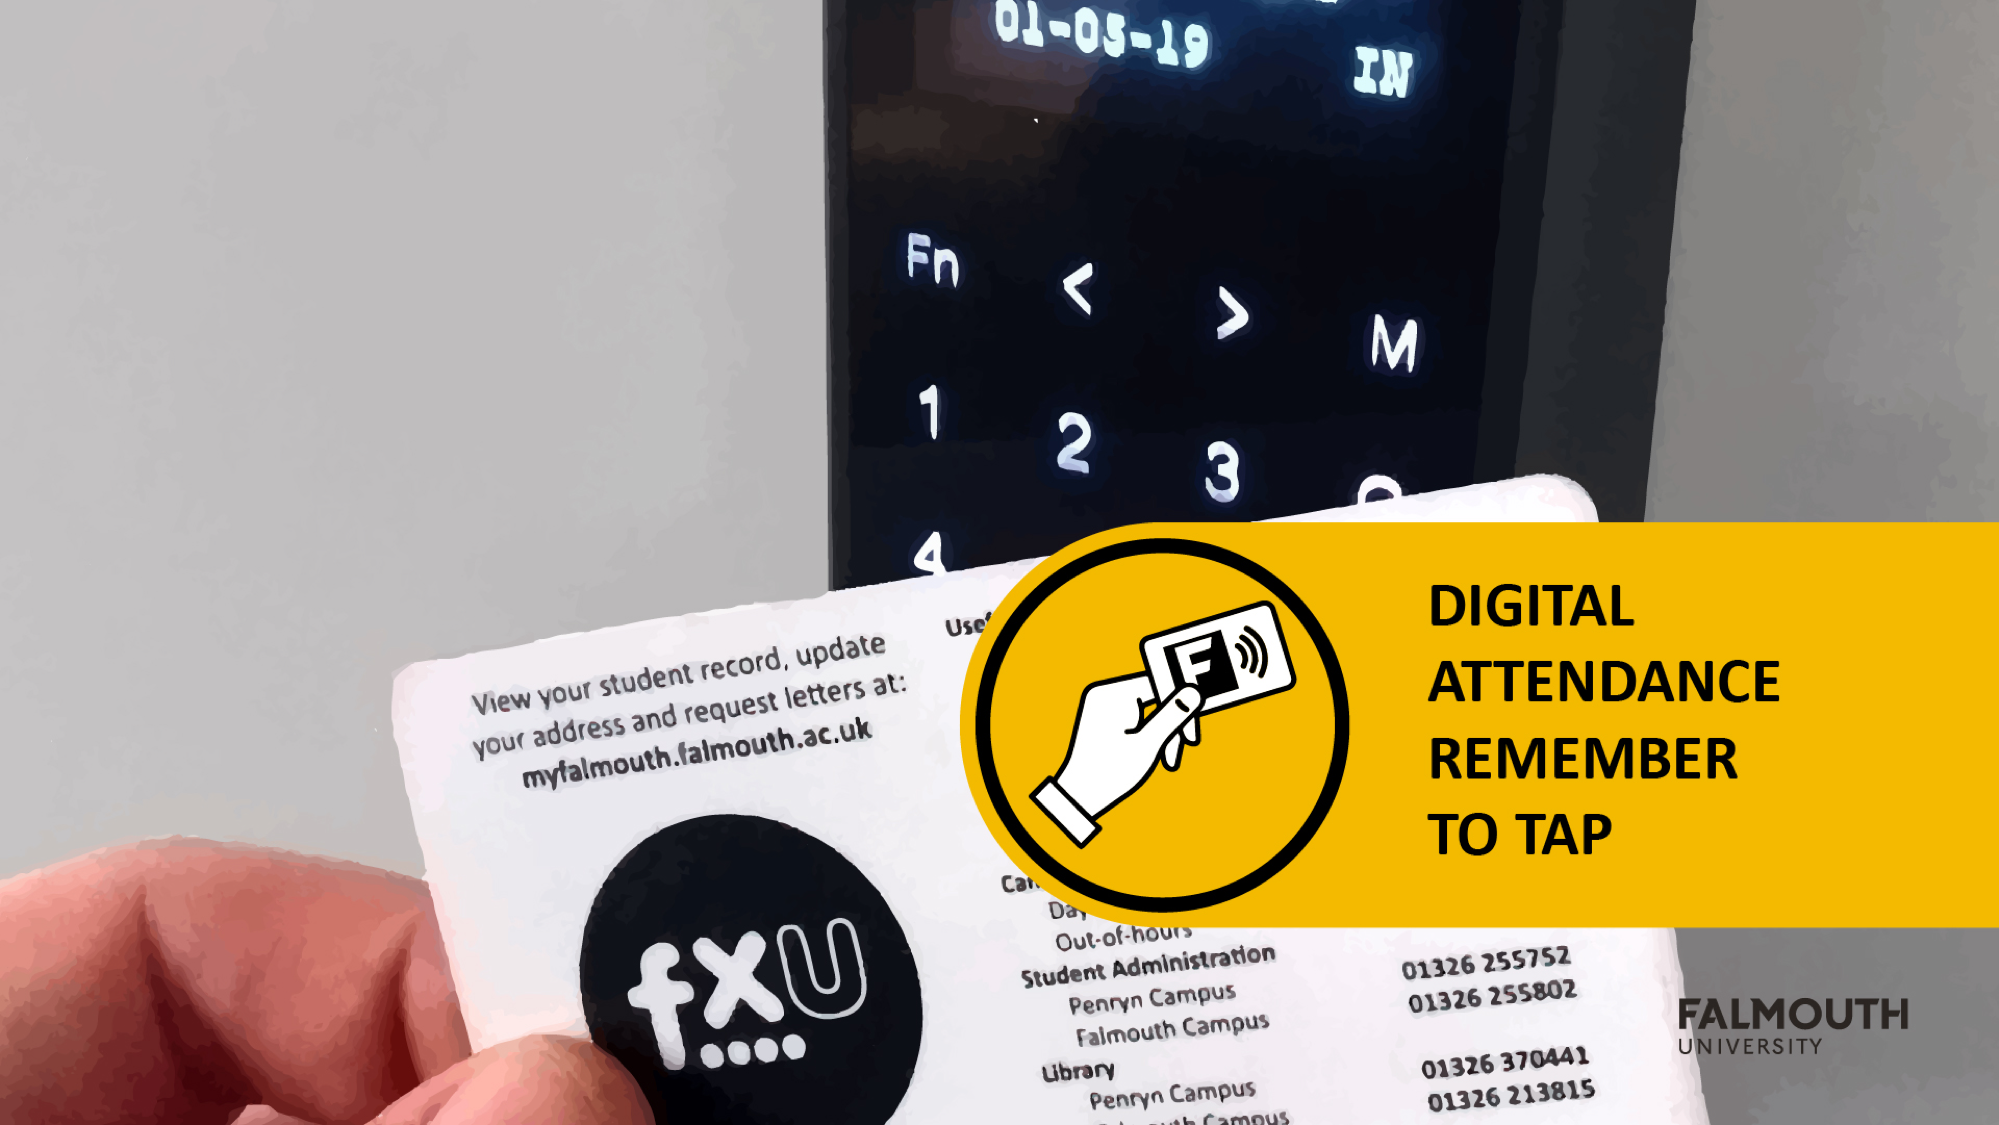
\includegraphics[width=1.0\textwidth]{sign-in}
\end{frame}

\frame{\titlepage} 


\begin{frame}{Today's agenda}
	\begin{itemize}
		\item Prototype Due Date
		\item Design Goals
		\item Physical Prototyping
	\end{itemize}
\end{frame}

\begin{frame}{First Prototype - DIY}
\begin{center}
	\Huge{Due Today 5pm!}
\end{center}
\end{frame}

\part{Design Goals}
\frame{\partpage}

\begin{frame}{Intro}
	\begin{itemize}
		\item As a designer it is important to have sort of intent
		\item It is important to think of what kind of response you want from your audience
		\item 
	\end{itemize}
\end{frame}

\begin{frame}{Design Pillars}
	\begin{itemize}
		\item Something about your game that everything should revolve around
		\item Establish once the your are in production
		\item Better for larger games
		\item Traditionally this is focused on mechanics but try to think about emotions you want at the core of your game
	\end{itemize}
\end{frame}

\begin{frame}{Audience/Player Experience Goals}
	\begin{itemize}
		\item Less rigid than Design Pillars
		\item You should focus on the emotional journey you want the player to go on
		\item This should inform your design process at all times
		\item If a feature detracts from this experience then cut it
	\end{itemize}
\end{frame}

\begin{frame}{Constraints}
	\begin{itemize}
		\item Constraints are drivers for creativity
		\item As a Designer you will bump up against them
		\item The Friction caused will cause you to think of ideas to beat the constraints
		\item Or to bend them to your will and use them in your design
	\end{itemize}
\end{frame}

\begin{frame}{Game Design Macro}
	\begin{itemize}
		\item Monolithic Design Docs are not very useful
		\item No-one in the team reads them
		\item Document is slow to evolve
		\item Game Design Macro attempts to capture the high level design 
	\end{itemize}
\end{frame}

\begin{frame}{Game Design Macro}
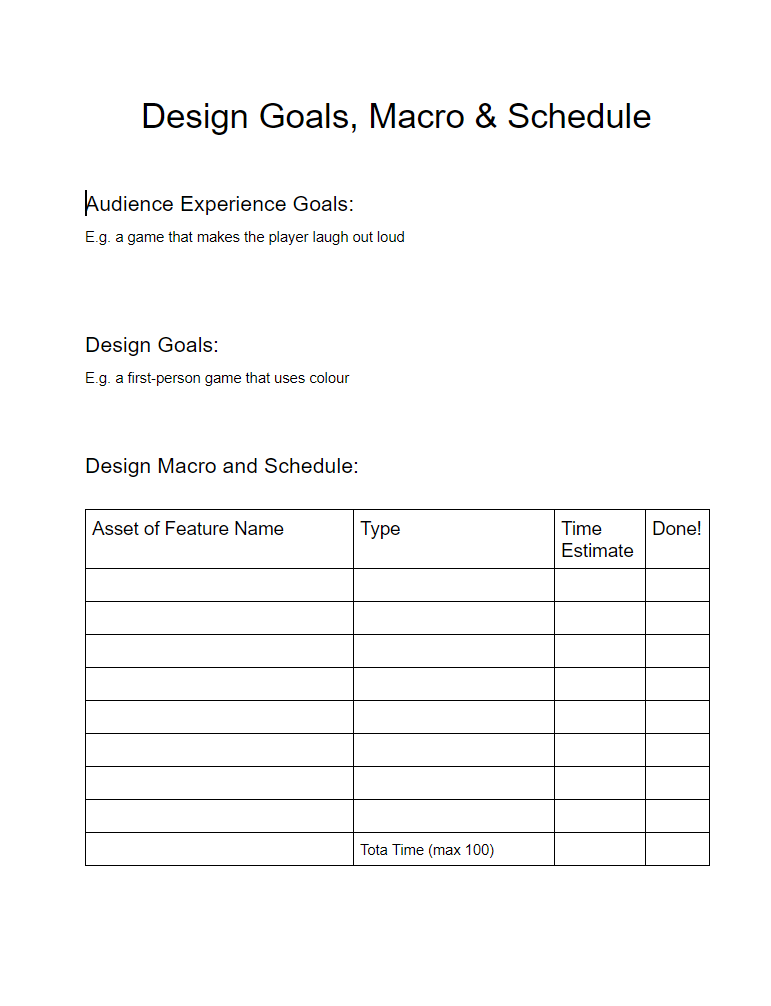
\includegraphics[width=1.0\textwidth]{game_design_macro}
\end{frame}

\begin{frame}{One Page Designs}
	\begin{itemize}
		\item First described by Stone Librande (Riot Games) 
		\item Instead of writing a Design Doc
		\item You write a series of one page design docs which detail some aspect of the game
		\item This could be a map, a visual description of the combat, relationship between characters
	\end{itemize}
\end{frame}

\begin{frame}{One Page Designs}
	\begin{center}
		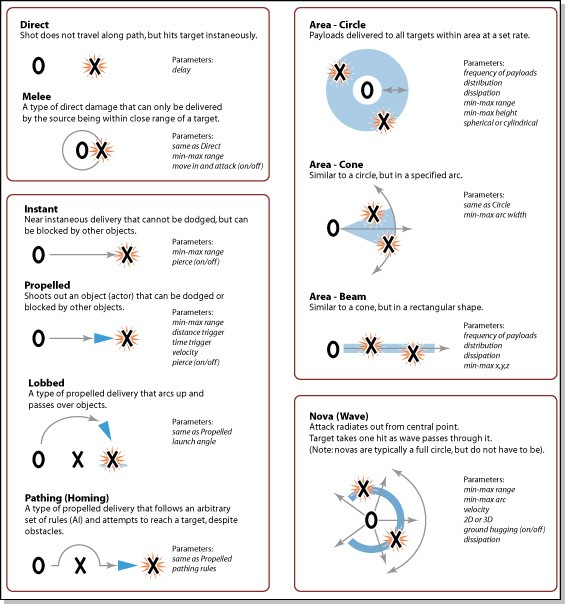
\includegraphics[width=0.7\textwidth,height=0.7\textheight]{combat_diagram}
	\end{center}
\end{frame}

\begin{frame}{One Page Designs}
	\begin{center}
		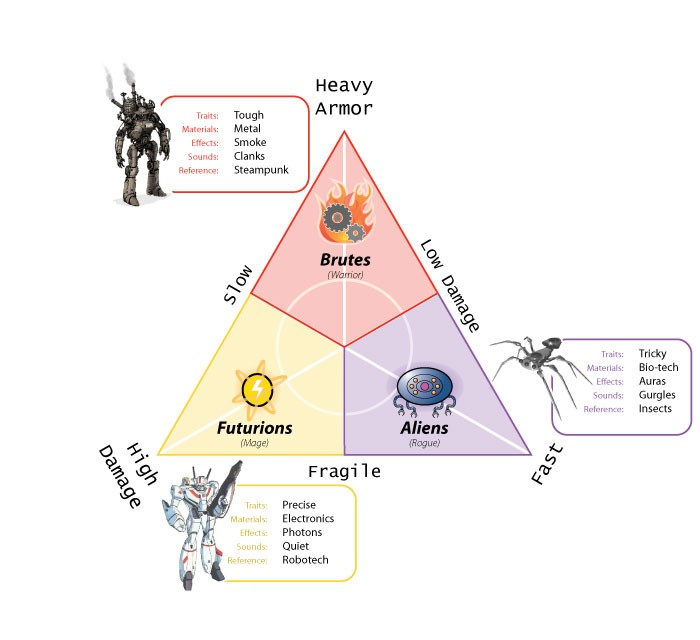
\includegraphics[width=0.7\textwidth,height=0.7\textheight]{unit_diagram}
	\end{center}
\end{frame}

\begin{frame}{One Page Design Template}
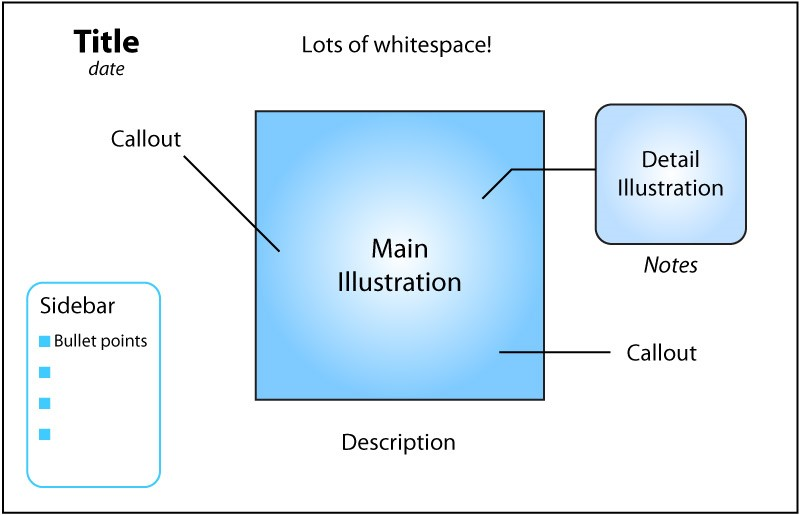
\includegraphics[width=1.0\textwidth]{one_page_design_template}
\end{frame}

\begin{frame}{One Page Design Benefits}
\begin{itemize}
	\item Forces a complete understanding of the game
	\item Forces a concise design
	\item Highlights relationships
	\item Aids problem solving
\end{itemize}
\end{frame}

\part{Paper Prototyping}
\frame{\partpage}


\begin{frame}{Second Prototype - Theme Announcement}
\begin{center}
	\Huge{Due Friday 5pm on Week 5!}
\end{center}
\end{frame}

\begin{frame}{References}
\end{frame}

\end{document}
